\section*{Introduction}

	The risk-free yield curve is a theoretical concept that plays a very important role in a wide range of financial applications.  
	It is crucial component of the pricing and valuation processes in different contexts: accounting, risk-management, etc. 
	Since there is no such thing as a risk-free asset in the real market,\footnote
{
After the world financial crisis this convention is widely accepted (reference to BIS congress papers).
}
risk-free rates cannot be observed directly. 
	The construction of risk-free curve always requires some assumptions and model describing prices of financial instruments, so any outcome depends on a data chosen, a model built and numerical methods applied.
	The typical structure of yield curve construction problem is presented on Figure \ref{problem_structure}.

\begin{figure}[h]
	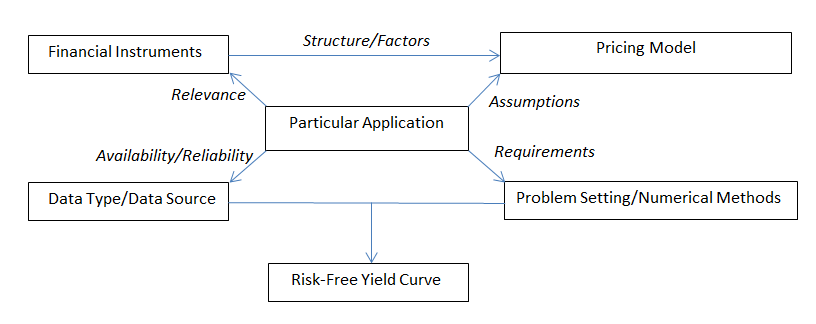
\includegraphics[width=\textwidth]{problem_structure}
	\caption{Structure of risk-free yield curve problem.}
	\label{problem_structure}
\end{figure} 

%	Indeed, all parts of the problem are interconnected. 

	There are some generally accepted (fundamental) properties that any estimate of the risk-free yield curve is expected to have, such as non-negative forward rates.
	 At the same time, a particular application determines special requirements to the construction methodology and special features of curve estimate itself. 
	In this paper, we consider construction of risk-free yield curve for the valuation long-term obligations, e.g. life insurance or pension liabilities, and refer in this context to the ``best estimate''\footnote
{
	According to the Solvency II regulation, the best estimate is the one component of so-called technical provisions. 
	Another component is the risk margin that reflects cost of providing a necessary capital amount to support obligations over their lifetime. 
	Together best estimate and risk margin represent an amount theoretically needed to transfer the obligations to another insurance undertaking (see Article 77 of  Solvency II Directive (Directive 2009/138/EC)).
}  
 which is calculated as a present value of projected future cash flows arising from undertaking's obligations and discounted with a relevant risk-free curve.

	Long-term obligations are typically stretched far beyond maturities prevailing in the market and the valuation requires extrapolation of the interest rates implied by market data, so liabilities value depends on assumptions about how long-term rates behave. 
	As the example on Figure \ref{yield_curve_example} shows, up to the certain maturity (for example, 20 years) rates are mainly determined by observed (and reliable) prices of relevant financial instruments, while  the rest of the curve is supposed to be constructed from special considerations. 
	It is worth to note that rates fitted to market data become ``starting point'' for extrapolated ones, so together with chosen assumptions they determine the whole extrapolated trajectory.  
	
\begin{figure}[h]
	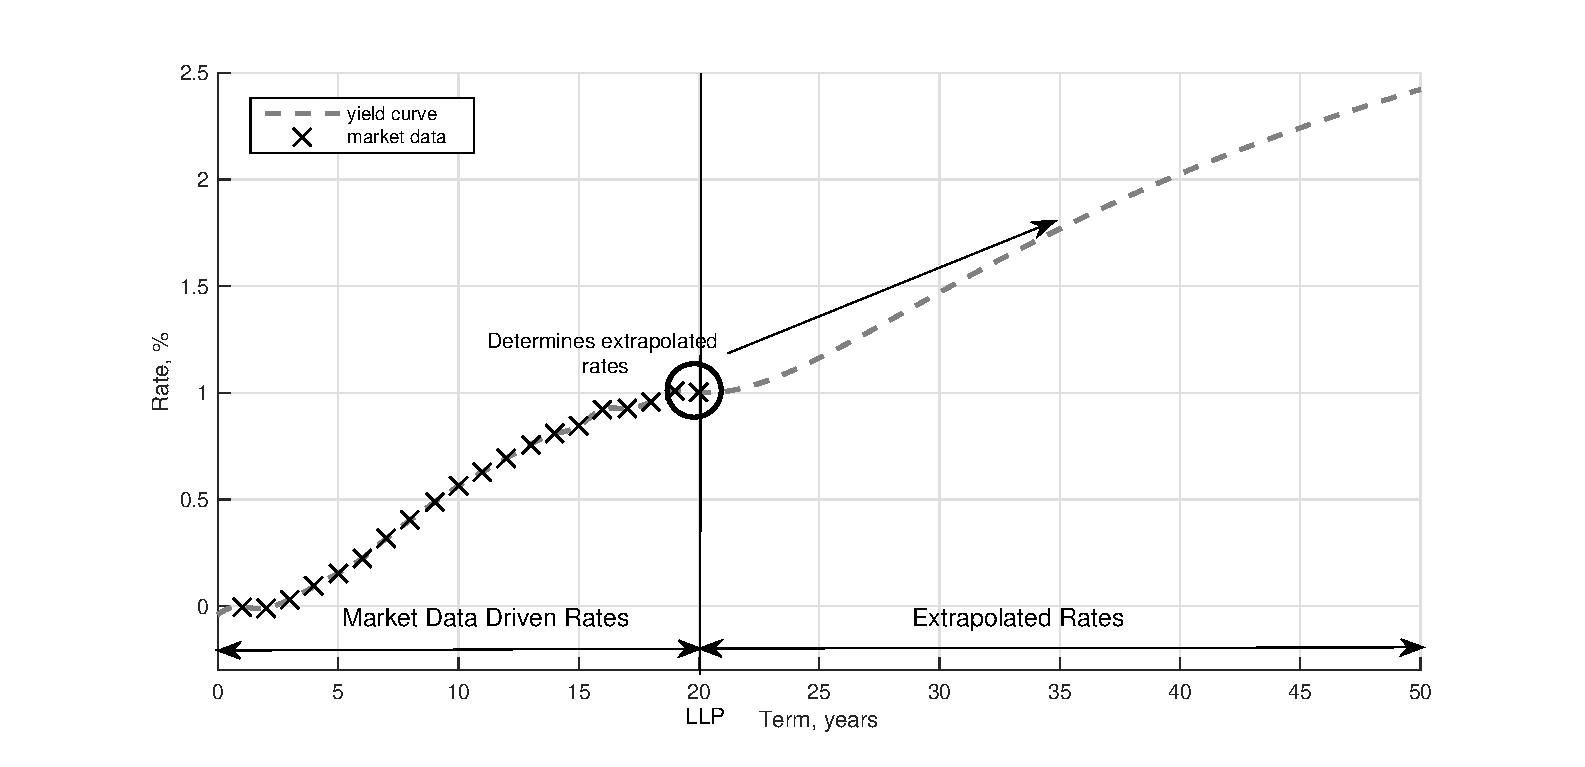
\includegraphics[width=\textwidth]{yield_curve_example}
	\caption{Example of yield curve for valuation of long-term liabilities.}
	\label{yield_curve_example}
\end{figure} 

	 The liabilities value of insurance undertaking corresponds to the value of its assets attributed to fulfill obligations to its policyholders. Thus, risk-free curve in use plays determining role in sharing the undertaking's wealth between policyholders and shareholders. 
	In particular, all other things being equal, the greater interest rates benefit shareholders.
	Therefore, an issue of objectivity and fairness of methodology of risk-free yield curve construction is a key problem related to the protection of policyholders' interests. 
	This aspect raises concerns especially with respect to an extrapolated part of the curve, as there is less certainty about how it should be constructed, but the way it is done may significantly impact obligations value.
%	The similar rationale is applicable in regard to intergenerational solidarity, i.e. the risk-sharing among different policyholders or pension fund participants (see Vellekoop, 2015).
	In this regard, note that the market-consistency principle is generally accepted as the objectivity criterion for rates determined by market data.

%\begin{figure}[h]%{0.49\textwidth}
%	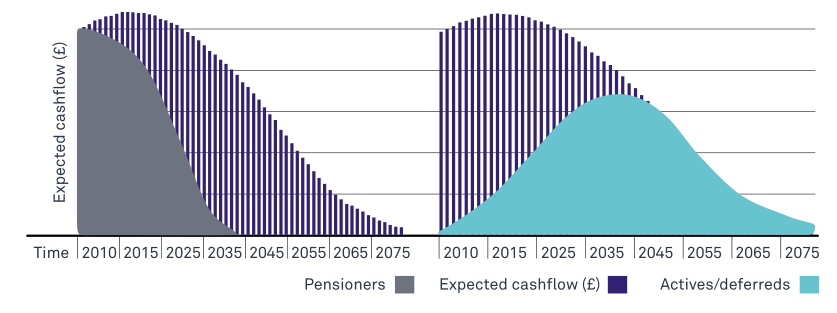
\includegraphics[width=\textwidth]{profile}
%	\caption{Typical cash flow profile.}
%	\label{fig_zero_nonparam}
%\end{figure}

	Final but, probably, most important aspect corresponding to long-term liabilities valuation relates to opportunities of asset liability management (ALM) and hedging. 
	From the perspective of ALM, undesirable volatility is the volatility that cannot be hedged out. 
	On the one hand, this means that the risk-free curve should not generate a significant artificial and unhedgeable volatility of technical provisions. 
	On the other hand, the risk-free rate should not over-stabilize liabilities value, since it leads to unhedged exposures on the asset side of the balance sheet.  
	Both they create excessive variability of accounting and performance information which does not adequately represent an economic condition of an undertaking. 
	In particular, the recital 30 of Directive 2014/51/EU says that ``the relevant risk-free interest rate term structure should avoid artificial volatility of technical provisions and eligible own funds and provide an incentive for good risk management.''

	Different market data can be used for risk-free curve construction. 
	As mentioned above, the currently prevailing convention is that no financial instrument should be considered as risk-free, so, depending on context, various instruments and wide range of proxies of risk-free rate are used in practice: to name a few, Libor or Euribor rates, Interest Rates Swaps (IRS) and Overnight Indexed Swaps \footnote
{
 Apparently, OIS is the least risky instrument developed today.
}
(OIS),  repo rates, sovereign bonds are most often used. 
	Not only risks associated with particular instrument matter but availability and reliability of its price data for relevant maturities. 
	The relevance of instruments for the business that risk-free curve is applied should also be taken into consideration.
	
	What instruments suit best for the risk-free curve estimation in actuarial context was widely and fairly long discussed question.
	In particular, implementing the Solvency II Directive, EIOPA
%	\footnote
%{
%One of the three financial supervises bla-bla-bla....previously CEIOPS bla-bla-bla
%}
 has been making its choice between sovereign bonds and interest rate swaps.  
	Finally, Delegated regulation (EU) 2015/35 (2015) declared that swap rates are preferable over bond prices arguing that in general the swap markets are substantially liquid, deep and transparent (DLT) and prescribed to use interest rate swaps for estimating the risk-free term structure\footnote
{
Prior to the risk-free curve construction swaps rates are supposed to be adjusted to the spread of Euribor over OIS. In EIOPA's methodology this procedure is referred to as credit risk adjustment (CRA). For more details see EIOPA Technical Standards (2017). 
}.
	Postulating superiority of swap market rates over bond market prices, European regulation, however, doubts that rates of all tenors are reliable in regard of risk-free curve estimation. Therefore, taking liquidity into account, it limits longest tenor involved in risk-free rates derivation. This tenor is called last liquid point (LLP) and for euro is set equal to 20 years legislatively, regardless of the fact that the DLT analysis undertaken by EIOPA indicates that 25 year and 30 year interest rate swaps for euro are also DLT.\footnote
{
 For different currencies LLP is set separately by EIOPA. EIOPA also defines what tenors shorter than LLP should be exclude from constructing risk-free rates due to low market liquidity. 
}  
	 As for sovereign bond prices, they should be used only for those relevant to European market currencies for which liquid, deep and transparent swap markets do not exist.  
	
	The decision by European regulation to use swap rates in order to derive risk-free rates one may find debatable. 
	Indeed, interest rate swaps are standardized and quite liquid instruments covering wide range of maturities and data on their prices and specifications are very convenient for yield curve construction. 
	But on the other hand,  interest rate swaps may be less relevant to the business of insurers and pension funds, because their portfolios are heavily invested in bonds of high credit quality.\footnote
{
{\color{red} It may not be an argument, because, although insurers' and funds' portfolios are primarily invested in bonds, undertakings actively use interest rate derivatives for duration management and constitute a significant share of swap users. }.
}
	Apart from that, (LIBOR-like) rates underlying interest rate swaps can be subject to manipulations, as they present average indicative rate (without commitment) announced by panel banks.\footnote
{ 
It was first noticed by Jean-Francois Borgy in his unpublished paper in 2007 and subsequently confirmed by the LIBOR scandal [see the Federal Reserve Working Paper by Hou and Skeie (2014)].
}
	Therefore, extracting yield curve out of financial instruments which prices can be manipulated by their nature may be not in line with interests of policyholders and pension fund participants. In particular, our paper shows how correct choice of methodology helps to overcome this unpleasant property of interest rate swap data.
	
	There is no doubt that bonds are very important for funding insurance and pension obligations, but dealing with bond data is more delicate in comparison with interest rate swaps. Bonds are less standardized and issued by issuer of different credit quality\footnote
{
In particular, in eurozone  sovereign bonds issued by different countries have different credit quality. 
} 
which is priced differently. 
	Moreover, the bonds carrying comparable credit risks may be different in term of liquidity and have different liquidity premiums. 
	Thus, besides risk-free rates, many factors determining bond prices have to be taken into account. 
	It may take not only building a more complicated model, but involve other instruments into consideration. 
	For example, see Smirnov, Lapshin, Kurbangaleev (2017) for the methodology of constructing risk-free term structure using sovereign bonds issued by eurozone members and respective CDS contracts.
%	In this section we give an introduction to the problem of risk-free yield curve constructions. 
%	It includes  structure of the problem and description of its key elements. 
%	It also contains a review of previous research and discussions related to the problem and their critical analysis.  
	
	What determines the yield curve beyond the market-traded terms is still open question from both theoretical and practical perspectives. 
	The theoretical literature derives the behavior of long-term rates from arbitrage-free  term structure models. 
	In general, inferences from particular model depend on  arbitrage definition, market completeness assumption and trading constraints and stochastic properties of risk factors. 
	One of the pioneering and general results of that kind is the well-known theorem by Dybvig, Ingersoll and Ross (1996) showing that in arbitrage-free market the long-term zero-coupon rates can never fall. 
	Since then this result has been generalized and extended multiple times. 
	Brief but extensive overview of such papers can be found in de Kort (2017). 
	Although the most of such models are internally consistent, the inferences from them can hardly be verified by market data, so those models at most are impractical for extrapolation purposes. 
	Therefore, for practical purposes it is customary to adopt general economic or engineering considerations in order to extrapolate market yield curve. 	
 
	Basic extrapolation principles regarding implementation of Solvency II Directive are formulated in Directive 2014/51/EU. 
	It states that constructed forward curve should converge to the so-call ultimate forward rate (UFR). 
	The technical requirements to UFR and how forward curve should converge to it were clarified in Delegated regulation (EU) 2015/35.  
	In particular, Article 47 of the regulation requires the UFR to be stable over time and be revised only due to changes in long-term expectations.
	It also states that UFR is supposed to be determined by expectation of the long-term real interest rate and expected inflation.\footnote
{
	In fact, the regulation proceed from the rational expectation principles regarding the UFR determination.  
}
	The methodology for deriving UFR was developed by EIOPA in 2017 and shell be implemented in 2018.\footnote
{
For more information see EIOPA-BoS-17/072.
}    
	As for the convergence of forward curve, according the Article 46 forward rates should smoothly converge to the UFR over 40 years after last liquid point.
	
	In this regard, the idea of UFR has been critically assessed by Vellekoop (2015) published in Network for Studies on Pensions, Aging and Retirement. The author describes the role that UFR and its modeling play in wealth and risk sharing among stakeholders and risk management. He concludes that there is neither empirical evidence nor theoretical reason to think that ultimate forward rate should be constant. He also argues that the methodology proposed by EIOPA will complicate the risk management and hedging practice because hedging regulatory risk highly contradicts economic hedging of interest risk. 
	
	In order to construct the risk-free yield curve EIOPA has developed special methodology based on Smith--Wilson fitting method (see Smith and Wilson (2001)). 
	This spline method finds the smoothest forward curve that simultaneously exactly reproduces prices of selected market instruments and converges  to set UFR over predefined horizon with certain degree of precision.\footnote
	{
	Formal derivation of Smith-Wilson solution can be found in Gach (2016).
	} 
	The property of Smith-Wilson method that is often seen as an advantage is that its solution is explicitly expressed, so it is rather tractable and easy to implement, reproduce and apply either to swap rates or to bond prices. 
	
\bigskip
	
{\color{blue} Insert mathematical description of SW if needed!!!}

\bigskip

%	Since 2015 EIOPA calculates and monthly publishes their estimates for all currencies relevant for European insurance and reinsurance undertakings. 
%		The methodology is based on Smith-Wilson applied to fitting forward curve to market data (prices of IRS or relevant bonds) and used to extrapolate this result beyond last tenor traded in the market.  

	The shape of yield curve is determined by:

\begin{enumerate}
	\item market data inputs;
	\item ultimate maturity beyond which interest rates are supposed to be extrapolated (last liquid point, LLP);
	\item long-term level of forward rate (ultimate forward rate,  UFR);
%	\footnote
%	{
%	Looks like  academics and experts are against having fixed level of UFR arguing that it is unjustified and impractical (See Vellekoop, 2015). 
%	}
	\item speed of convergence of forward rates to UFR (parameter $\alpha$). 
\end{enumerate}

%{\color{red} [If I get everything right, pension funds are not under influence of Solvency II and different approaches are applicable to valuation of pension liabilities.]}

%	In this paper we focus on robustness issue of EIOPA methodology and propose its modifications overcoming them. 
	There are series of drawbacks that constantly raise concerns among practitioners and academics.   	

	First of all, for some inputs the method can produce negative discount factors. 
%	Important to note that Smith-Wilson is a approximate solution to the correctly set problem.  
	This artifact was emphasized by EIOPA (CEIOPS at that time) itself as a one of the main disadvantages of Smith-Wilson method in QIS 5 on extrapolation method carried out in 2010. 
	 Since for the most inputs method works properly, while negative discount factors usually correspond to low $\alpha$ values,  EIOPA set a constraint on convergence speed factor $\alpha$ in order to avoid negative discount factors.
	 So $\alpha$ is supposed to be not less then 0.05.  
	 However, Lageral and Lindholm (2016) provides the real-case example how discount function extracted from Russian ruble swap rates by Smith-Wilson method on 16 December 2014 turns out to be negative beyond LLP (10 years) even for $\alpha > 0.05$.  
	 This paper also demonstrates that occurrence of negative factors correspond to a singularity in convergence criterion used in fitting with Smith-Wilson method.
	 The possibility of negative discount factors should be definitely considered as a serious shortcoming of the Smith-Wilson method since it argues against the conceptual soundness of the method and reliability of the results it produces.
	 
	Another unpleasant and highly criticized property of Smith-Wilson method is an extreme sensitivity to the inputs in LLP and LLP-1.
	In particular, it makes value of all cash flows expected to occur beyond LLP to be heavily dependent on the input in LLP and LLP-1.
	This sensitivity is essentially a sequence of the fact that all forward rates beyond last liquid point are primarily (but not solely) determined by forward rate in LLP,  UFR and predefined horizon over which forward curve is supposed to converge to UFR with a given degree of precision.
	Moreover, inputs in LLP-1 and LLP affect liabilities value in opposite directions. 
	In particular, this phenomenon is presented in Ovtchinnikov (2014).
	All other things being equal, an increase of swap rate in LLP raises the rates beyond LLP, so cash flows dated after LLP will be discounted heavier and value of liabilities will decrease.
	In contrast, an increase in swap rate in LLP-1 will  likely generate decline in forward rate in LLP that, in its turn, will case decline of all forward rates beyond LLP resulting in greater discount factor for long-dated cash flows.
	One of the earliest works pointed at this ware paper by Kocken, Olden Kamp and  Potters (2012).
	The authors argue that great sensitivity to the swap rate in LLP and LLP-1 will drastically increase demand for such swaps, since these instruments became main hedging tool for long-term liabilities of insurance undertakings. 
	They conclude that hedging practice of undertakings trying to manage duration of their long-term obligations will distort liquidity of swap market in those segments, making them effectively illiquid.
	The sensitivity around LLP was also mentioned as an issue in several responses  to EIOPA's consultation paper EIOPA-CP-16-008 in 2017.\footnote
	{
	See, for instance, responses by Actuarial Association of Europe (AAE) or Association of British Insurers (ABI) on consultation webpage: https://eiopa.europa.eu/Pages/Consultations/EIOPA-CP-16-008-Discussion-Paper-on-the-Review-of-Specific-Items-in-the-Solvency-II-Delegated-Regulation.aspx.
	}
	
	Note that sensitivity of yield curve and liabilities value to inputs of other maturities is rather moderate, but exact fitting may accumulate the mutual effect of small changes over time and amplify an effect of rate changes in LLP and LLP-1 on the rest of the curve. 
	In particular, it means that result of any valuation carried out with yield curve constructed with Smith-Wilson method will be sensitive even to small errors in data.
	 It all leads to the overall instability of the method, so regardless of the nature of market data the value of long-term liabilities becomes significantly and artificially volatile. 
	It is also worth to note that any result obtained with such non-robust method should not be considered as satisfactory, as it cannot be validated using an analogous data from alternative source.
	{\color{red}Eventually, it is difficult to adopt a set of potential scenarios for results by obtained with non-robust method in order to assess risk or to carry out stress-test.}
	
	In order to overcome the sensitivity problem Kocken, Olden Kamp and  Potters (2012) suggest to let market data beyond LLP determine the way forward rate converges to UFR.
	Their approach is essentially is Smith-Wilson method when market data up to LLP is  fitted, but beyond the LLP the yield curve is constructed from weighted average of UFR and market forward rates beyond LLP.
	Thus, market swap rates beyond LLP affect extrapolated part of the curve but since more weight is assigned to UFR for longer maturities, forward rates still converge to UFR. 
	To keep their approach in a line with EIOPAs methodology they derive weighting scheme from Smith-Wilson method.
	In more detail this their approach has been studied by Rebel (2012) whose work, in particular shows, that it result in smoothing of sensitivity profile and reducing overall sensitivity level.
	As one can justify, this approach was initially adopted by De Nederlandsche Bank for pension fund regulation.
	Later, De Nederlandsche Bank has modified this approach by introducing variable ultimate forward rate which was defined as the 10 year moving average of the twenty year historical market forward rate.
	By this step regulator aspires to ensure market-consistency of approach and to eliminate undesirable effect of unanticipated discrete adjustments in UFR on technical provisions of pension funds.
	A comparison of EIOPA's methodology, already mentioned Dutch approaches and Swedish methodology for valuation pension liabilities was carried out in Broeders, de Jong and Peter (2016).
	The authors analyzes these techniques from the perspectives of predictability of UFR adjustment, speed of convergence to UFR, hedgability and potential market impact. 
	They concluded that all three domestic approaches are slightly preferable over EIOPAs methodology. 
	Finally, de Kort and Vellekoop (2016) consider UFR as a free parameter in fitting Smith-Wilson curve to the market data. Slightly reformulating the problem and applying smoothing criterion to forward rate function, they derive the UFR as optimal asymptotic level corresponding to the smoothest discount function. Note that authors put the Smith-Wilson problem in a context close to the Hull-White short rate model, so properties fitted curve are close to the properties of term structure implied by the model and UFR can be interpreted as a mean-reverting level.
	
	Although from purely practical point of view the proposed solutions surely demonstrate enhancement over EIOPA's methodology, they are clearly an ad-hoc and lack for conceptual soundness. 
	They also only partially solve the problem with non-robustness of Smith-Wilson method by limiting effect of forward rate in LLP on further trajectory of forward curve, while forward rate in LLP itself remains extremely unstable and sensitive to small changes in market data. 

	
	In this paper we bla-bla-bla....
	
		
	
	
%	Consistent stress-testing.
%	As an arbitrage can be defined different ways, the non-arbitrage principle is not straightforward. 
%	The particular condition also depends on assumptions about stochastic process driving basic variables of assets value and about market completeness. 

